%-------------------------------------------------------------------------------
% preferences
%-------------------------------------------------------------------------------
%
% \file        preferences.tex
% \library     Documents
% \author      Chris Ahlstrom
% \date        2015-08-31
% \update      2025-05-30
% \version     $Revision$
% \license     $XPC_GPL_LICENSE$
%
%     Provides the Menu section of seq66-user-manual.tex.
%
%-------------------------------------------------------------------------------

\section{Edit / Preferences}
\label{sec:edit_preferences}

   The \textbf{Edit / Preferences} dialog has a number of tabs.

   \textbf{Preferences} provides a number of settings in one
   tabbed dialog, shown in the figures that follow.
   It allows one to set MIDI clocking, MIDI Input, display tweaks, minor
   playback options, and some JACK parameters.

   Configuration items implemented in \textbf{Preferences} are
   incoming MIDI events to control the sequencer;
   outgoing MIDI events to light up the display on a MIDI controller;
   what keys are mapped to functions;
   how the mouse works, and a few others.
   The MIDI and Key controls, far more numerous than in \textsl{Seq24}, have
   been consolidated into a 'ctrl' file and are fairly easy to edit with a text
   editor.
   \textsl{Seq66} does not support the 'fruity' mouse mode at this time.
   If you want it, ask us!

\subsection{Edit / Preferences / MIDI Clock}
\label{subsection:edit_preferences_midi_clock}

   \textbf{Note}:
   \textsl{The MIDI Clock tab is sometimes difficult to click on.}
   We are not sure why.  It seems to be theme-dependent.
   In some things the tab thumb changes color when it can work.
   Just keep clicking in various locations in the tab,
   or use the \texttt{Alt-C} key.
   Weird.

   The \textbf{MIDI Clock} tab provides a way to set MIDI clocking for
   the available MIDI output busses.
   It configures the output busses for MIDI clock and data.
   It shows the devices that can play music.
   The items that appear in this tab depend on:

   \begin{itemize}
      \item What MIDI devices are connected to the computer.
         MIDI controllers, USB MIDI cables, applications with virtual
         ports, and other connected devices will add MIDI
         output devices (ports) to the system.
         This list will generally match the output of \texttt{aplaymidi -l}
         or \texttt{aconnect -lio}.
      \item The setting of the "manual-ports" option, which tells
         \textsl{Seq66} to set up virtual MIDI ports.
         It is enabled by the
         \texttt{-{}-manual-ports} command-line option or the
         \texttt{[manual-ports]} section of the
         \texttt{qseq66.rc} configuration file,
         or in the \textbf{MIDI Input} tab described below.
      \item The setting of the \textsl{Seq66}-specific
         "reveal ALSA ports" option,
         \texttt{-{}-reveal-ports} command-line option or the
         \texttt{[reveal-ports]} section of the
         \texttt{qseq66.rc} configuration file.
   \end{itemize}

   If \texttt{-{}-manual-ports} is on, this list shows the virtual
   MIDI output busses that \textsl{Seq66} can drive.
   One needs to use a JACK or ALSA MIDI
   connection application to connect a device on each of those outputs.
   (But \textsl{Seq66} itself can connect to another instance of
   \textsl{Seq66}. See \sectionref{sec:recording_seq_to_seq}.

   The fact that the the buss names can
   start with different numbers, depending on the system setup, can complicate
   the playing of MIDI in this manner.  Also, the 'usr' configuration file can
   change the visible names of the ports to match specific equipment attached
   to the ports.

\begin{figure}[H]
   \centering 
   \includegraphics[scale=0.50]{main-menu/edit/preferences/midi_clock_tab.png}
   \caption{MIDI Clock (Output) Tab}
   \label{fig:midi_clock_tab}
\end{figure}

   This diagram shows the tab for configuring MIDI output and clocking
   features.

   \begin{quotation}
      \textbf{Tip}:
      With some Qt themes, it is difficult to activate this tab by clicking
      because there is little or no sensitive area on the tab.
      In this case, click \texttt{Alt-c} once or twice.
   \end{quotation}

   Port-mapping is the default, and when active, the names of the ports
   in the map are shown in this pane.
   If there are more than about a dozen
   output ports in the system, then a vertical scrollbar appears.
   The following elements are present in this tab:

   \begin{enumber}
      \item \textbf{Ports and Clocking}
      \item \textbf{Clock Start Modulo}
      \item \textbf{Buss Override}
      \item \textbf{MIDI I/O Maps}
      \item \textbf{Create (maps)}
      \item \textbf{Clear (maps)}
      \item \textbf{MIDI Control Out Bus}
      \item \textbf{Meta Events}
      \item \textbf{Client Name:ID/UUID}
      \item \textbf{Restart Seq66!}
   \end{enumber}

   \setcounter{ItemCounter}{0}      % Reset the ItemCounter for this list.

   \itempar{Ports and Clocking}{output!ports and clocks}
   \index{output ports}

   This table shows the available MIDI outputs and their status.
   If the set of system MIDI devices and software devices has changed since
   the last run, this list could be in error.  Restart the application
   and see if it is now correct.  Currently, there is no way to edit the list
   except in the 'rc' file.

   The \textbf{Ports and Clocks} table contains the following elements,
   although some can be removed by specifying the
   \texttt{port-naming = short} option in the 'rc' file.
   This option is preferred when using JACK.

   \begin{enumber}
      \item \textbf{Index Number} (optional)
      \item \textbf{Client Number} (optional)
      \item \textbf{Port Number} (optional)
      \item \textbf{Buss Name}
      \item \textbf{Port Disabled}
      \item \textbf{Off}
      \item \textbf{On (Pos)}
      \item \textbf{On (Mod)}
      \item \textbf{Clock Start Modulo}
   \end{enumber}

   The format of the left side of the entry listing is like the following
   when the port-naming option is "long", and the
   MIDI subsystem is ALSA):

   \begin{verbatim}
      [5] 128:4 yoshimi:input
       ^  ^   ^ ^       ^
       |  |   | |       |
       |  |   | |        ----- Port/buss name
       |  |   |  ------------- Client name
       |  |    --------------- Port/buss number
       |   ------------------- Client number
        ---------------------- Index number
   \end{verbatim}

   \setcounter{ItemCounter}{0}      % Reset the ItemCounter for this list.

   \itempar{Index Number}{midi clock!index number}
   \index{index number}
   The number in square brackets is an ordinal indicating the position
   of the output buss in the list.
   For all practical purposes in \textsl{Seq66}, it \textsl{is} the
   buss/port number.  This number can be stored in a pattern in order to have
   the pattern's output go to that buss.  
   This is true even if port-mapping is in place.
   \index{port!mapping}
   \index{buss!mapping}
   \index{port!override}
   \index{buss!override}
   It can be used with the \texttt{-b},
   \texttt{-{}-buss}, or \texttt{ -{}-bus} options to redirect
   \textsl{all}
   pattern output to that buss, useful if only one buss is active or the
   \textsl{Seq66} patterns route to non-existent busses.
   (See \sectionref{subsubsec:introduction_sets_buss_override},
   and \sectionref{subsubsec:usr_file_user_midi_settings}.)

   \itempar{Client Number}{midi clock!client number}
   \index{client number}
   The number that precedes the colon is the "client number".
   It is useful mainly in ALSA, where clients can have numbers like "14",
   "128", "129", etc.  For native JACK mode, it matches the index number.

   \itempar{Port Number}{midi clock!port number}
   \index{port number}
   The number that follows the colon is the "port number".
   It is useful mainly in ALSA.
   For native JACK mode, it matches the index number.

   \itempar{Buss Name}{midi clock!buss name}
   \index{port name}
   \index{midi clock!port name}
   These labels indicate the output busses (ports) available.
   \textsl{Seq66} does not access devices by name, but by port number.
   However, a port-map can be created to make it possible to find the correct
   buss / port number by name lookup.

   \itempar{Port Disabled}{midi clock!port disabled}
   The \textbf{Port Disabled} clock choice marks an output port
   that the user does not want to use or that the operating system
   (\textsl{Windows} \smiley)
   is locking or disabling.
   Normally, this inaccessible port would cause \textsl{Seq66} to exit.
   With the port disabled, the inaccessible port is ignored.
   This feature also shows when a port-map cannot find a device in the system's
   device list.
   When the \textsl{Windows} version of \textsl{Seq66}
   (\texttt{qpseq66.exe}) is first started, it may error out.
   It will then write a default \texttt{qseq66.rc}
   or \texttt{qpseq66.rc} configuration file,
   which can be examined to find the offending buss, which can then be
   marked in the normal 'rc' file as disabled.

   \itempar{Off}{midi clock!off}
   Disables the MIDI \textsl{clock} function for the given output buss.
   MIDI output is still sent to those ports, and
   each port that has a device connected to it will play music.
   Some synthesizers may require this setting.

   \itempar{On (Pos)}{midi clock!on (pos)}
   MIDI clock will be sent to this buss.
   MIDI Song Position and MIDI Continue will be sent if playback starts
   at greater than tick 0 in Song mode.  Otherwise, MIDI Start will be sent.
   Note: In case of trouble, see
   \sectionref{subsec:alsa_testing}.

   \itempar{On (Mod)}{midi clock!on (mod)}
   MIDI clock will be sent to this buss.
   MIDI Start will be sent, and clocking will begin
   once the Song Position has reached the start modulo of the specified size
   (see the next item's description).
   This setting is used for gear that does not respond to Song Position.

   Below the \textbf{Ports and Clocks Table} are more configuration elements.

   \setcounter{ItemCounter}{0}      % Reset the ItemCounter for this list.

   \itempar{Clock Start Modulo (ticks)}{midi clock!clock start modulo}
   This value starts at 1 and ranges up to 16384, and defaults to 64 ticks.
   It is used by the \textbf{On (Mod)} setting discussed above.
   It is the \texttt{[midi-clock-mod-ticks]} option in the \textsl{Seq66}
   'rc' file.

   \itempar{MIDI I/O Port Maps}{midi clock!port maps}
   If checked (the default), then port-mapping is employed.
   This makes it a bit easer to manage MIDI devices across systems and to store
   the port/buss numbers in each pattern.
   Note that both input and output port mappings are activated by this
   checkbox.
%  If changed, the \textbf{Restart Seq66!} button is enabled.

   \itempar{Create (maps)}{midi i/o!port mapping}
   \index{port mapping}
   \index{port!mapping}
   Pressing this button saves the current set of MIDI I/O ports to sections in
   the 'rc' file.  These sections can be enabled in order to support
   port-mapping in subsequent runs of \textsl{Seq66}.
   Generally, after pressing this option, one will want to stop
   \textsl{Seq66}, rearrange the clock and input maps in the
   'rc' file with a text editor, back up this file in a safe place,
   and restart \textsl{Seq66}.

   \itempar{Clear (maps)}{midi i/o!remove mapping}
   \index{remove mapping}
   \index{port! remove mapping}
   Pressing this button removes the port mapping.
   \index{restart!manual}
   Once done, either restart \textsl{Seq66} or go to the \textbf{Session}
   tab and click the \textbf{Restart} button.
   (See \sectionref{subsec:concepts_reload_session}.)

   \itempar{MIDI Control Out Bus}{midi control!output buss}
   \index{midi control!output}
   Use this control to select the output bus used to display
   application-automation status, loop status, and mute-group status.
   Requires a \textsl{reload session} to take effect.
   The number of the buss is stored in the 'ctrl' file named in
   \sectionref{subsection:edit_preferences_session},
   as the value of \texttt{output-buss}.
   If port mapping is enabled (now the default),
   the nick-name of the bus is stored instead of the number.
   The device on the output buss must have a corresponding
   'ctrl' file output section properly defined.

   \itempar{Meta Events}{midi clock!meta events}
   \index{tempo-track-number}
   This section consists of the following items:

   \begin{enumerate}
      \item \textbf{Tempo track number}
      \item \textbf{BPM Precision}
      \item \textbf{Set Tempo Track}
   \end{enumerate}

   \textbf{Tempo track number}
   allows the user to move the tempo track from pattern 0 to
   another pattern.  Changing this option is not recommended, since track 1 (0)
   is the official track for tempo events, but \textsl{Seq66} allows the
   user to record tempo events to another track.  \textsl{Seq66} will
   process tempo events in any pattern.

   \index{usr!bpm-precision}
   \textbf{Precision}
   allows setting the number of digits past the decimal point to 0, 1, or 2.
   This is also a 'usr' setting.
   See \sectionref{subsubsec:usr_file_user_midi_settings}.
   The BPM (tempo) is stored in the MIDI file multiplied by 1000 to accommodate
   the decimal places.

   \textsl{Set Tempo Track}
   Enabled when a valid tempo track number is given.
   It makes the tempo track official if it is not zero anymore.

   \itempar{Client Name:ID/UUID}{client ID}
   This read-only text field shows two things:

   \begin{enumerate}
      \item \textbf{Client Name}.
         This is the name of the client under ALSA or JACK.  It defaults to
         \texttt{seq66}, but it can be altered by the command-line option
         \texttt{-{}-client-name} or by a session manager.
         Each instance of Seq66 run under ALSA will have a different client ID.
      \item \textbf{ID/UUID}.
         Under ALSA, the client number (client ID) is shown.
         Under JACK, the UUID that JACK assigned to \textsl{Seq66} is shown.
   \end{enumerate}

   \itempar{Restart Seq66!}{restart}
   Certain changes require a \textsl{Seq66} restart, unfortunately.
   When enabled, clicking this button does not exit \textsl{Seq66},
   but it does cause all of the internal mechanisms to be recreated
   from scratch.

%  \index{todo!manual alsa gui option}
%  There is currently no user-interface item corresponding to the "manual-ports"
%  command-line and 'rc' configuration file option.
%  We should rename this option to "virtual" eventually.

\subsection{Edit / Preferences / MIDI Input}
\label{subsection:edit_preferences_midi_input}

   To set up \textsl{Seq66} to record MIDI from devices such as
   controllers and keyboards, the output of the ALSA MIDI recording
   command-line \texttt{arecordmidi -l} is relevant.
   Something like that listing appears in the Input tab:

\begin{figure}[H]
   \centering 
   \includegraphics[scale=0.50]{main-menu/edit/preferences/midi_input_tab-2.png}
   \caption{MIDI Input Tab}
   \label{fig:midi_input_tab}
\end{figure}

   Port-mapping is the default, and when active, is shown in this pane.
   If there are more than about a dozen
   input ports in the system, then a vertical scrollbar appears.

   Any item checked allows \textsl{Seq66} to record MIDI from that source,
   which must be connected to this input port.

   \textbf{Warning:}
   \index{warnings!usr config}
   \index{usr config}
   If the 
   \texttt{[user-midi-bus-definitions]} value in the 'usr' configuration file
   is non-zero, and the
   corresponding number of
   \texttt{[user-midi-bus-N]} settings are provided, then
   the list of existing hardware will be ignored, and those values will be
   shown instead.
   This feature can be overridden with the
   \texttt{-{}-reveal-ports} (\texttt{-r}) option.
   If you define these sections, they should match your
   hardware exactly, and your hardware should not change from session to
   session (or port-mapping should be enabled).
   If the "auto ALSA ports" option is turned on, via the \texttt{-a} or
   \texttt{-{}-auto-ports} option, then
   the input ports from the system are shown.

   \setcounter{ItemCounter}{0}      % Reset the ItemCounter for this list.

   \itempar{Input Buses}{input buses}
   \textbf{Input Buses} delineates the MIDI input devices as noted above.

   \itempar{MIDI Control Input Bus}{midi control!input buss}
   \index{midi control!input}
   Use this control to select the input bus used for MIDI control automation of 
   application actions, loop actions, and mute-group actions.
   Requires a \textsl{reload session} to take effect.
   The number of the buss is stored in the 'ctrl' file named in
   \sectionref{subsection:edit_preferences_session},
   as the value of \texttt{control-buss}.
   If port mapping is enabled (now the default),
   the nick-name of the bus is stored instead of the number.

   \itempar{Input/Output Options}{I/O options}
   \index{input options}
   \textbf{Input/Output Options} adds further refinements to MIDI input and
   output.
   It has the settings described below.

   \itempar{Record-by-Bus}{record!by bus}
   \index{input by buss}
   \textbf{Record into patterns by buss}
   causes MIDI input from multiple busses to be distributed to
   each sequence according to MIDI input buss number.
   If set, it overrides the record-by-channel setting.

   \itempar{Record-by-Channel}{record!by channel}
   \index{input by channel}
   \textbf{Record into patterns by channel}
   causes MIDI input with multiple channels to be distributed to
   each sequence according to MIDI output channel number.

   Only one of these record-by options can be enabled at the same time.
   The record-by-buss option takes precedence.

   When these options are disabled,
   the normal recording behavior dumps all data into the current
   sequence, regardless of channel or buss.
   See \sectionref{sec:recording}, which describes recording in more detail.

   \itempar{Input/Output Virtual Ports}{ports!virtual}
   \textbf{Use virtual (manual) I/O ports}
   Virtual ports are called "manual ports" because the connects
   generally need to be made manually.
   This option
   allows for configuration of the manual-ports option from within the
   user-interace. 
   Also included are settings for the number of manual input and output ports.
   (In \textsl{Seq24}, 16 output and 1 input port were created.)
   Once the option is enable
   A \textsl{reload session} (see \sectionref{subsec:concepts_reload_session})
   is necessary for this option to take effect.

   \itempar{Virtual Ports Auto-Enable}{ports!virtual auto-enable}
   \textbf{Auto-enable virtual I/O ports}
   If set, the ports are all automatically enabled upon a restart.
   The following figure shows that a large number of virtual ports can be
   defined.

\begin{figure}[H]
   \centering 
   \includegraphics[scale=0.95]{main-menu/edit/preferences/midi_input_tab-virtual.png}
   \caption{MIDI Virtual Inputs}
   \label{fig:midi_input_tab_virtual}
\end{figure}

   Note that the user is responsible for connecting the virtual MIDI ports,
   using something like \textsl{aconnect} (ALSA) or
   \textsl{qjackctl} (JACK).

\subsection{Edit / Preferences / Keyboard (removed)}
\label{subsection:edit_preferences_keyboard}

   Unlike \textsl{Seq24}, \textsl{Seq66}
   \textsl{does not} provide an options tab for
   setting up the keyboard.
   There are just too many new keystroke-automation functions to fit
   in a configuration dialog box.
   The default keyboard mappings follow \textsl{Seq24} fairly well,
   but add a large number of additional controls;
   around 96 keystroke slots would need to be provided!
   The keystroke and MIDI controls are consolidated, and are easy to change by
   editing the appropriate 'ctrl' configuration file, stored in one of the
   following directories, depending on
   the operating system:
   
   \begin{verbatim}
         /home/username/.config/seq66/qseq66.ctrl           (Linux)
         C:/Users/username/AppData/Local/seq66/qpseq66.ctrl (Windows)
   \end{verbatim}

   There are also some extended examples present in the \textsl{Seq66}
   \texttt{data/linux} and
   \texttt{data/samples} directory.
   Also see \sectionref{sec:launchpad_mini}.
   For more information on keystrokes, see
   \sectionref{subsec:kbd_mouse_keyboard_control}.

   One useful enhancement, though "costly", would be support of MIDI Learn.
   Currently the only "learnable" items are the mute groups.

\subsection{Edit / Preferences / Mouse (removed)}
\label{subsection:edit_preferences_mouse}

   Unlike \textsl{Seq24}, \textsl{Seq66}
   \textsl{does not} provide an options tab for
   the mouse-interaction method.
   It is not supported in \textsl{Seq66}...
   the \textbf{Fruity} interaction method is not available;
   only the \textbf{Seq24} interaction is available.
 
\subsection{Edit / Preferences / Display}
\label{subsection:edit_preferences_display}

   This dialog provides a few odds and ends to enhance the user-interface.
   Some of these items (plus a few more) can be configured by editing the 'usr'
   file.

\begin{figure}[H]
   \centering 
   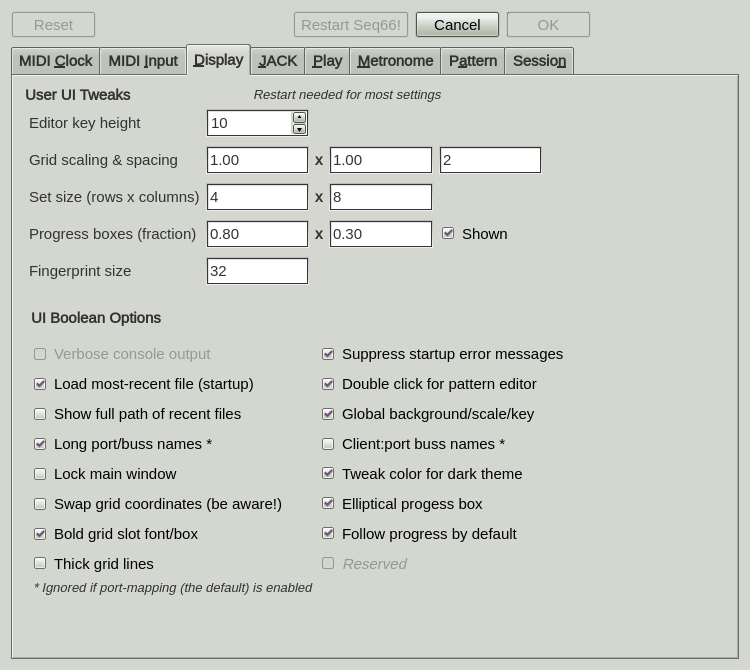
\includegraphics[scale=0.50]{main-menu/edit/preferences/midi_display_tab.png}
   \caption{Display Options}
   \label{fig:midi_display_tab}
\end{figure}

   Note: The \textbf{Thick grid lines} option does not appear in this
   figure.

   \setcounter{ItemCounter}{0}      % Reset the ItemCounter for this list.

   \itempar{Editor Key Height}{key height}
   This option affects the pattern editor's piano roll.  Smaller means a wider
   range of notes can be shown.  There are also
   \textbf{-},
   \textbf{0}, and
   \textbf{+} buttons in the pattern editor that provide
   vertical zoom.

   \itempar{Grid scaling \& spacing}{window scaling}
   These three items set scale factor for width and height of the main window,
   and adjust the spacing between the grid slots..
   The lowest scale factor is 0.5, and the largest scale factor is 3.0.
   For the smallest window, the smallest practical values are 0.85 x 0.60.
   The spacing unit is pixels.

   \itempar{}{set-size}
   Provides a way to change the set size.  The default is
   \textbf{4 x 8}
   (rows by columns), but we intend to support
   \textbf{4 x 4},
   \textbf{8 x 8}, and
   \textbf{12 x 8}
   as well.

   \textbf{Warning}:
   A different set size alters the 'ctrl' file layout radically.
   We still have to work through all the implications of changing the set size,
   so back up your configuration and proceed with caution!

   \itempar{Progress Boxes}{progress-box size}
   Provides a way to change the size of the progress box in each button.
   Values are width and height fractions (up to 1.0) re the button size.
   This is a 'usr' option.

   \itempar{Progress Box Shown}{progress-box shown}
   If the \textbf{Shown} check-box
   is \textsl{unchecked}, then the progress boxes and pattern color are not
   shown.
   This is a 'usr' option.

   \itempar{Fingerprint Size}{fingerprint size}
   This value, if set from 32 to 128, indicates the number of events above
   which a "fingerprint", rather than every note, will be drawn.  It can
   save some CPU time in drawing the grid.  If set to 0, the whole
   pattern is drawn, no matter how long the pattern is.

   In the \textbf{UI Boolean Options} section are some more options
   from the 'usr' file:

   \begin{itemize}
      \item Verbose console output. (Read only).
      \item Load most-recent file (startup).
      \item Show full path of recent files.
      \item Long port/buss names.
      \item Lock main window.
      \item Swap grid coordinates.
      \item Bold grid slot font/box.
      \item Thick grid lines.
      \item Suppress startup error messages.
      \item Double click for pattern editor.
      \item Global background/scale/key.
      \item Client:port buss names.
      \item Tweak color for dark theme.
      \item Elliptical progress box.
      \item Follow progress by default.
      \item \textsl{Reserved}. (For future expansion).
   \end{itemize}

   \itempar{Verbose Console Output}{verbose}
   This boolean makes more output appear if \textsl{Seq66} is run from a
   console/terminal. It will also increase the amount of data logged to the log
   file, if activated. It is only a temporary setting, just like
   its command-line counterpart, \texttt{--verbose}; when
   \textsl{Seq66} exits, the setting remains false.

   \itempar{Load Most Recent File (startup)}{load most-recent}
   If checked, the file at the top of the \texttt{[recent-files]}
   list in the 'rc' file is loaded at startup.

   \itempar{Show Full Path of Recent Files in Menu}{full paths}
   The full path of each file in the \texttt{[recent-files]} list
   is shown in the menu.  Although they can be uncomfortably long, they can
   show files that have the same name, but in different directores.

   \itempar{Long Port/Buss Name}{buss names!long}
   \index{buss names!short}
   Controls how much port information is shown in the clocks and input
   listings.  For the "portmidi" (e.g. \textsl{Windows})
   implementation, keep this option checked.

   \itempar{Lock Main Window}{main window!lock}
   This item makes the window non-resizable after startup.

   \itempar{Swap Grid Coordinates}{grid!swap coordinates}
   Normally, \textsl{Seq66} displays the pattern and mute-groups grids
   where the pattern numbers increase fastest downward.
   Some might prefer to have pattern numbers increase fastest rightward.
   This setting make the patterns show in the more conventional manner.

   \textbf{Warning}:

      \begin{itemize}
         \item This setting requires the 'ctrl' file to be rewritten
            if one want to preserve the normal layout for the pattern hot-keys
            and the mute-group hot-keys.
         \item This setting has not been rigorously tested, so be prepared for
            some issues to report.
      \end{itemize}

   A 'ctrl' file for the swapped setting is provided
   in \texttt{qseq66-swapped.ctrl} in the \texttt{data/linux}
   directory, but it might not be completely correct yet.

   \itempar{Bold Grid Slot Font/Box}{grid!bold}
   \index{font!bold}
   \index{progress bar!thick}
   This setting makes the font in the live grid bold, and it allows
   make the progress-bar thick in the grid and in the Live and Song piano
   rolls.
   It is the same as the \texttt{progress-bar-thick = true} option in the 'usr'
   file. See \sectionref{subsubsec:usr_file_user_interface_settings}.

   \itempar{Thick Grid Lines}{grid!thick}
   This option makes some lines in the pattern and song grid-panes
   stand out more. Try it and see what is preferable.

   \itempar{Suppress startup error messages}{quiet}
   Unlike the verbose setting, this one is sticky.
   It prevents the display of error prompts at startup.
   It is useful when the system keeps flagging the same problem,
   it cannot be fixed, and can be ignored.
   It is \textsl{not} the opposite of "verbose".

   \itempar{Double click for pattern editor}{grid!bold}
   \index{double-click!pattern slot}
   If set, a double-click on a grid button brings up the pattern for editing.
   Disable it if the effect is confusing.

   \itempar{Global background/scale/key}{globals!background etc.}
   \index{global pattern setting!background}
   \index{global pattern setting!key}
   \index{global pattern setting!scale}
   If set, setting the background sequence, scale to show, or the key of the
   track will apply to all pattern windows that are opened.

   \itempar{Client:port buss names}{buss!naming}
   \index{bus!naming}
   If checked the MIDI engine's "client:port" numbers are shown in the port
   listings.

   \itempar{Tweak Color for Dark Theme}{theme!dark}
   In dark themes, some interface items might be difficult to see.
   This option replaces some icons with brighter icons.
   Another option is to create a palette file.

   \itempar{Elliptical Progress Box}{grid!elliptical}
   This bit of eye candy merely makes the live grid slot progress box elliptical.
   If the \textbf{Progress Boxes} width an height fractions are equal,
   the progress box is a circle.

   \itempar{Follow Progress By Default}{progress!default}
   This item can be turned off if one does not want the pattern or song
   editors to scroll as playback occurs.
 
\subsection{Edit / Preferences / JACK}
\label{subsection:edit_preferences_jack}

   This tab sets up JACK transport, if \textsl{Seq66}
   was built with JACK support (\textsl{Linux} only).

\begin{figure}[H]
   \centering 
   \includegraphics[scale=0.50]{main-menu/edit/preferences/midi_jack_tab.png}
   \caption{Edit / Preferences / JACK}
   \label{fig:midi_jack_tab}
\end{figure}

   The main sections in this dialog are:

   \begin{enumber}
      \item \textbf{JACK Transport/MIDI}
      \item \textbf{JACK Start Mode}
      \item \textbf{JACK Transport Connect and Disconnect}
      \item \textbf{JACK Server Settings}
   \end{enumber}

   \setcounter{ItemCounter}{0}      % Reset the ItemCounter for this list.

   \itempar{Transport/MIDI}{jack sync!transport/midi}
   These settings are stored in the 'rc' file settings group
   \texttt{[jack-transport]}.
   This items collects the following settings:

   \begin{itemize}
      \item \textbf{Jack Transport}.
         \index{JACK!transport}
         Enables slave synchronization with JACK Transport.
         The command-line option is \texttt{-{}-jack-transport}.
         The behavior of this mode of operation is perhaps not quite
         correct.  Even as a slave, \textsl{Seq66} can start and
         stop playback.
         Note that this option cannot be disabled via the mouse if the
         \textbf{Transport Master} option is enabled.  Disable that one first.
      \item \textbf{Transport Master}.
         \index{JACK!transport master}
         \textsl{Seq66} will attempt to serve as the JACK Master.
         The command-line option is \texttt{-{}-jack-master}.
         If this option is enabled the \textbf{JACK Transport} option is
         automatically enabled as well.
      \item \textbf{Master Conditional}.
         \index{JACK!master conditional}
         \textsl{Seq66} will fail to serve as the JACK Master if there is
         already a Master.
         The command-line option is \texttt{-{}-jack-master-cond}.
         If this option is enabled the \textbf{JACK Transport} option is
         automatically enabled as well.
      \item \textbf{Native JACK MIDI}.
         \index{JACK!native midi}
         This option is for the \texttt{qseq66} (Linux) version of
         \textsl{Seq66}.
         If set, MIDI input and output use native JACK MIDI,
         rather than ALSA.  However, if JACK is not running on the
         system, then \texttt{seq66} will fall back to ALSA mode.
         (However, if \texttt{jackdbus} is running, but the JACK engine is not,
         then a couple of non-working manual ports are created.  To be fixed in
         the future.)
         The command-line option is \texttt{-{}-jack-midi}
         or \texttt{-{}-jack}.
      \item \textbf{JACK Auto-Connect}.
         \index{JACK!auto-connect}
         This option has been true for a long time in \textsl{Seq66}, and
         non-configurable.  Now it can be turned off, in order to let the user
         or a session manager make the connections, even when not using
         manual/virtual ports.
   \end{itemize}

   \begin{quotation}
      \textbf{Tip}:
      Seq66 generally works better as JACK Master than JACK Slave.
   \end{quotation}

   If one makes a change in the JACK transport settings, it is best to
   then press the \textbf{JACK Transport Disconnect} button, then the
   \textbf{JACK Transport Connect} button.
   Another option is to restart
   \textsl{Seq66}... the settings are automatically saved when
   \textsl{Seq66} exits.

   \itempar{JACK Start mode}{jack sync!start mode}
   This item collects the following settings, also stored in the 'rc' file
   settings group \texttt{[jack-transport]}.

   \begin{itemize}
      \item \textbf{Live Mode}.
         \index{JACK!live mode}
         \index{live mode}
         \index{non-playback mode}
         Playback will be in live mode.  Use this option to allow muting and
         unmuting of patterns.  This option might also be called "non-song
         mode".
         The command-line option is \texttt{-{}-jack-start-mode 0}.
      \item \textbf{Song Mode}.
         \index{JACK!song mode}
         \index{song mode}
         \index{playback mode}
         \index{performance mode}
         Playback will use only the Song Editor's data.
         The command-line option is \texttt{-{}-jack-start-mode 1}.
   \end{itemize}

   \textsl{Seq66} also selects the playback modes
   according to which window started the playback.
   \textsl{The main window}, or pattern
   window, causes playback to be in live mode.  The user can arm and mute
   patterns in the main window by clicking on sequences, using their hot-keys,
   and by using the group-mode and learn-mode features.
   The song editor causes playback to be in performance mode, also known as
   "playback mode", or \textbf{Song} mode.

   \itempar{Connect}{jack sync!connect}
   Connect to JACK Sync.
   This button is useful to restart JACK sync when making changes to it,
   or when \textsl{Seq66} was started in ALSA mode.

   \itempar{Disconnect}{jack sync!disconnect}
   Disconnect from JACK Sync.
   This button is useful to stop JACK sync when making changes to it.
   JACK connection and disconnection are disabled during playback, but the
   buttons don't yet reflect that status.

   \itempar{JACK Server Settings}{jack server!settings}
   This read-only section shows the current settings of the JACK
   server, as much as possible.

\subsection{Edit / Preferences / Play Options}
\label{subsection:edit_preferences_play_options}

   This tab contains some disparate options ostensibly related to playback.

\begin{figure}[H]
   \centering 
   \includegraphics[scale=0.50]{main-menu/edit/preferences/midi_play_options_tab.png}
   \caption{Play Options}
   \label{fig:midi_play_options_tab}
\end{figure}

   \setcounter{ItemCounter}{0}      % Reset the ItemCounter for this list.

   \itempar{Resume Note Ons...}{edit!resume notes}
   \textbf{Resume Note Ons at start/stop or sequence toggle}
   allows notes that had already started
   to be resumed when playback resumes.

   \itempar{Use File's PPQN...}{edit!use file ppqn}
   \textbf{Use File's PPQN for Pre-Existing Files}, if checked, allows
   \textsl{Seq66} to run using the PPQn of the MIDI file rather than
   the default \textsl{Seq66} internal PPQN.
   This is the recommended option for most MIDI files.
   When this option is changed, the \texttt{-{}-user-save} option is turned on
   to preserve the setting when \textsl{Seq66} exits.

   \itempar{Default Seq66 PPQN...}{edit!default ppqn}
   \textbf{Default Seq66 PPQN for New or Converted Files}, if checked, allows
   the standard PPQN, 192 pulses/quarter-note, to be changed to discrete values
   from 32 to 19200.  Intermediate values, even oddball values, can be entered
   by typing the number directly.
   When this option is changed, the \texttt{-{}-user-save} option is turned on
   to preserve the setting when \textsl{Seq66} exits.
   If there is a MIDI file loaded, it is modified to use the new PPQN, and the
   user is prompted to save it at exit.
   Best to have a backup, just in case.

   \itempar{Sets Mode}{edit!sets-mode}
   This item determines how sets are handled.
   Recall that a set is a number of patterns (up to 4x8) in the pattern grid,
   and that the current set is the one visible in the pattern grid.
   The way sets work in \textsl{Seq66} is that, when a set is selected,
   all the patterns in it are loaded into what is called
   the "play-set".
   When play starts only, patterns in the play-set are handled.
   The \textbf{Sets Mode} option allows special handling of the play-set.

   \begin{enumerate}
      \item \textbf{Normal}.
         In this mode, only the current set's patterns can be unmuted.
         When switching to another set, the current set's patterns become
         muted, and the new set's patterns are shown, unmuted.
      \item \textbf{Auto-Arm}.
         Here, when the new set is loaded, it is immediately unmuted.
      \item \textbf{Additive}.
         With this option, when a new set is loaded, the previous set keeps
         playing. This allows a build-up of patterns in playback.
      \item \textbf{All Sets}.
         Here, all sets in the tune are loaded and unmuted at once.
         Try this mode with the \texttt{b4uacuse-stress.midi} file
         in the \textsl{Sequencer64} project.  It's a good test of
         \textsl{Seq66} and your hardware/software synthesizer!
   \end{enumerate}

   One can clear the out play-set, and set only the current set active, by
   clicking the exclamation point button to the left of the "Active" label at
   the bottom of the main windows.

\subsection{Edit / Preferences / Metronome Options}
\label{subsection:edit_preferences_metronome}

   This tab contains options for the "metronome" and
   "background recording" features:

\begin{figure}[H]
   \centering 
   \includegraphics[scale=0.50]{main-menu/edit/preferences/midi_metro_options_tab.png}
   \caption{Metronome Options}
   \label{fig:midi_metro_options_tab}
\end{figure}

   \setcounter{ItemCounter}{0}      % Reset the ItemCounter for this list.

   The metronome feature is enabled in the main live grid via a metronome
   button.
   The metronome is a standard \textsl{Seq66} pattern that is used
   for playback of the metronome, but it is never seen
   nor directly edited by the user.
   It is not saved with a song, so changing the metronome does not modify the
   song.
   The settings shown above are saved to a "metronome" section in the 'rc'
   file.
   The metronome is a pattern that first plays a main note once, and then
   plays "sub" notes for the rest of the measure.
   Here are the settings:

   \itempar{Beats/bar}{metronome!beats/bar}
   This setting sets the beats-per-measure for the metronome only.
   It currently does not affect the time-bar in the main window.
   Should it? There is a global beats/bar as well as beats/bar for
   each pattern.

   \itempar{Beat width}{metronome!beat width}
   This setting sets the beat width for the metronome only.
   The following settings are provided for the "main" note
   (the note that occurs on the beginning of the measure)
   and the "sub" notes (the notes that occur on each beat):

   \itempar{Patch}{metronome!patch}
   This item sets the program (patch) number for the note, which sets the
   instrument to play for the notes.
   We currently do not have a drop-down box to select the patch by name.
   The default patch is 0.
   As noted below, the default channel is 10, so this
   patch is the "Standard Drum Kit" for the device.
   Thus, by default the metronome can be implemented by two different
   drums.

   \itempar{Note}{metronome!note}
   This item provides the note value to be played.  Recall that 60 is the same
   as "middle C".  By default, the main note is 75, the "Clave" for the drum
   kit, and the sub note is 76, the "High Wood Block" for the drum kit.

   \itempar{Velocity}{metronome!velocity}
   This item provides the note velocity to be played, to provide an accent on
   the main note.

   \itempar{Length Fraction}{metronome!length fraction}
   The length of the notes are specified as a fraction of the beat width, and
   this value ranges from 0.125 to 1.0 to 2.0.
   If set to 0, the length is half of the beat width.

   \itempar{Reload Metronome}{metronome!reload}
   This button pauses playback (if playing),
   loads in the new metronome settings, and
   continues playing (if it was playing).
   It is \textsl{not} enabled when the status/configuration of background
   recording changes.

   \itempar{Metro Buss}{metronome!buss}
   This value selects the output MIDI device to use to play the metronome.
   It \textsl{must} be enabled in the \textbf{MIDI Clock} list.

   \itempar{Channel}{metronome!channel}
   This value selects the channel to use to play the metronome.

   \itempar{Record Buss}{recorder!buss}
   \index{background recorder}
   This value selects the input device to use to record events into the
   background pattern.
   Note that this device \textsl{must be enabled} in the \textbf{MIDI Input}
   buss list.

   \itempar{Thru Buss}{record!thru buss}
   This value selects the output MIDI device to use to play the incoming
   background record notes.  Otherwise they will not be heard.
   It \textsl{must} be enabled in the \textbf{MIDI Clock} list.

   \itempar{Thru Channel}{recorder!thru channel}
   This value selects the channel to use to play the recorded notes as
   they come in.

   We still have some more work to do to refine the metronome, the
   background recorder, and their configuration, pending user input.
   For more information about the metronome, see
   \sectionref{subsection:edit_preferences_metronome}.
%  For information on count-in background recording, see
%  \sectionref{subsection:edit_preferences_background_recording}.

\subsection{Edit / Preferences / Pattern}
\label{subsection:edit_preferences_pattern}

   This tab provides options for the status of newly-created patterns
   and for randomization of amplitude and jitter of time-stamps.

\begin{figure}[H]
   \centering 
   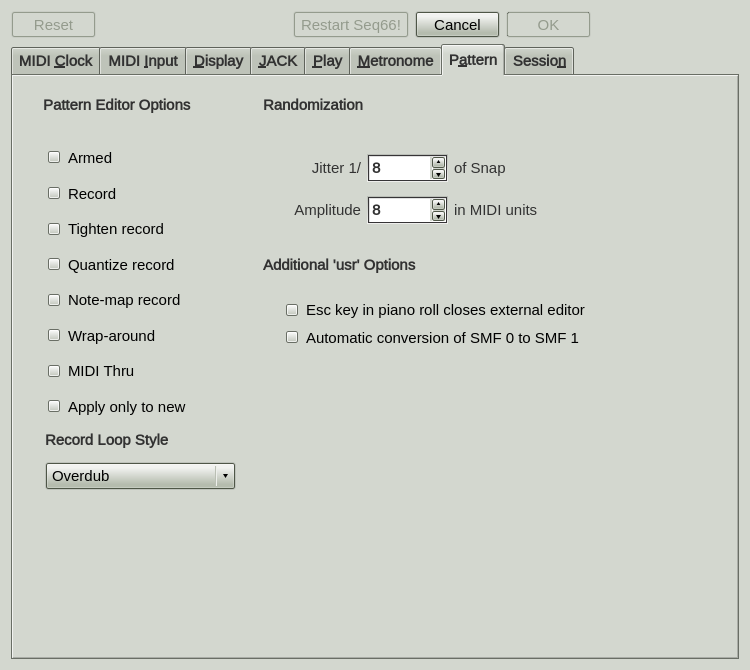
\includegraphics[scale=0.50]{main-menu/edit/preferences/midi_pattern_tab.png}
   \caption{Pattern Options}
   \label{fig:midi_pattern_options_tab}
\end{figure}

   \itempar{Pattern}{edit!pattern}
   \textbf{Pattern}
   This relatively new tab provides a way to configure the status of
   a newly-created pattern.
   It also provides a way to change the range of amplitude randomization
   and time jittering of events.

   The first section is \textbf{Pattern Options}.
   It defines the statuses of a newly-created or newly-opened pattern.
   This can be convenient for live-recording.
   The status setting are:

   \begin{itemize}
      \item \textbf{Armed}.
         This setting causes the pattern to be armed when a new pattern
         is created.
      \item \textbf{Record}.
         The new pattern starts in record mode.
      \item \textbf{Tighten record}.
         The new pattern starts in tightened (partly quantized) record mode.
      \item \textbf{Quantize record}.
         The new pattern starts in quantized record mode.
      \item \textbf{Note-map record}.
         The new pattern starts in note-mapping record mode.
         Notes are translated live via a 'drums' file, if set active
         in the 'rc' file.
      \item \textbf{Wrap-around}.
         The new pattern will allow prolonged notes to wrap around so
         that the Note Off event precedes the Note On event in the
         pattern loop.
      \item \textbf{MIDI Thru}.
         The new pattern starts with MIDI Thru enabled.
      \item \textbf{Apply only to new}.
         If check-marked, then the settings are applied only to
         newly-created patterns. Often one might not want to
         automatically record into an existing pattern, for example.
      \item \textbf{Record Style}
         This setting sets how record mode works for the pattern.
         \begin{itemize}
            \item \textbf{Merge}.
               As recording and looping proceeds, new events merge with
               the existing events.
            \item \textbf{Overwrite}.
               When the pattern loops back to its beginning, any
               existing events are deleted.
               A good way to try to get the right collection of notes.
            \item \textbf{Expand}.
               When recording as notes are recorded, the pattern expands to
               accomodate them.
               This results in a longer pattern than initially specified.
            \item \textbf{Oneshot}.
               Events are entered until the end is reached.
               Useful for recording stock patterns from a drum machine.
            \item \textbf{Oneshot Reset}.
               At the end of the specified length of the pattern,
               all events are cleared.
               Normal recording is set.
               Need to look into this as we cannot rememember all the
               details :-D.
         \end{itemize}
      \item \textbf{Apply to new only}.
         If checked, only a newly-created pattern will have the options
         above automatically applied.
   \end{itemize}

   The second section is \textbf{Randomization}.
   The range of randomization is based on a range parameter, and
   goes from -range to +range.
   The concept of jitter means that the time-stamps of recorded events
   are randomized slightly.
   The concept of randomization means that the amplitudes of events
   are randomized slightly.
   The randomization settings are:

   \begin{itemize}
      \item \textbf{Jitter}.
         This value is a jitter divisor.
         It sets the fraction of of the current snap value that
         is used as the range of jittering the time.
         For example, "8" means that the range is 1/8th of the snap value.
      \item \textbf{Amplitude}.
         This value is used for various data values.
         For Notes On (but not Notes Off), this parameter affects
         the range of amplitude variation, when amplitudes are
         the standard MIDI range, 0 to 127.
   \end{itemize}

   One minor issue, which we're still trying to work around, is that
   our various randomization algorithms seem biased to emit
   negative numbers.
   If one clicks in a pattern editor piano roll, types
   \texttt{Ctrl-A} to select all notes (and aftertouch)
   and types the \texttt{r} key repeatedly to randomize
   note amplitudes, the overall velocities slowly descend to 0.
   Still not sure what's wrong with \textsl{Seq66} randomization, 
   but it is only important if randomizing a large number of times.

   The next section is \textbf{Additional 'usr' Options}.
   It contains only one option at present,
   \textbf{Esc key in piano roll closes external editor}.
   If set (the default is false), then the \texttt{Esc}
   key can not only stop playing and exit paint mode, but
   can also close the pattern window.
   Be careful. It's your call.

\subsection{Edit / Preferences / Session}
\label{subsection:edit_preferences_session}

   This tab contains options related to session management and the
   configuration files.

   \setcounter{ItemCounter}{0}      % Reset the ItemCounter for this list.

\begin{figure}[H]
   \centering 
   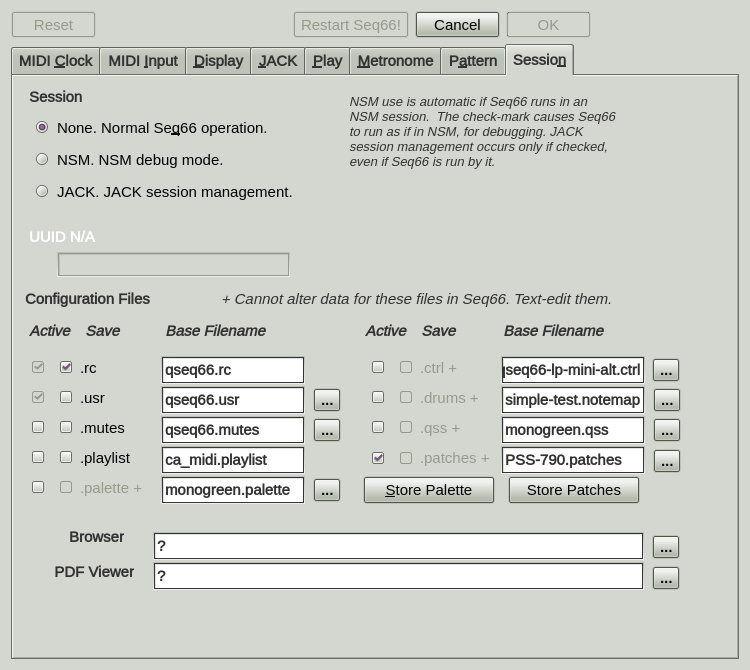
\includegraphics[scale=0.50]{main-menu/edit/preferences/midi_session_tab.png}
   \caption{Session Options}
   \label{fig:midi_session_options_tab}
\end{figure}

   This dialog has a couple of new items, to allow changing the web browser and
   PDF view to use.  See below.

   \setcounter{ItemCounter}{0}      % Reset the ItemCounter for this list.

   \itempar{Session}{edit!session}
   \textbf{Session}
   This tab provides for three modes of session management:  None, the
   Non/New Session Manager (NSM), and JACK Session management.
   None is the normal mode of operation, where the user has full control of
   where to put files, what other applications are to be run alongside
   \textsl{Seq66}, and what connections are to be made.

   NSM provides a rigorously-controlled session management, and directs
   \textsl{Seq66} what menu items to display, whether to hide the
   user-interface or not, where configuration files and MIDI files go, and what
   applications are run in a session. It can also (via \texttt{jackpatch}) keep
   a record of connections to reconstruct.

   JACK Session provides a location for file and a record of applications and
   connections, but otherwise lets the user mess things up.  It is
   provided because some people still use it.
   For more information about session management, see
   \sectionref{sec:sessions}.

   \itempar{UUID}{edit!UUID}
   \textbf{UUID} is a read-only field that shows any UUID that's relevant to a
   session. Normally has a value only in a \textsl{JACK} or
   \textsl{NSM} session.
   Also see the \textbf{Session} tab in the main window
   (\sectionref{sec:sessions}).

   \itempar{Configuration Files}{edit!configuration}
   \textbf{Configuration Files}
   shows the status of the configuration files.
   (See \sectionref{subsec:configuration_rc}).
   The 'rc' and 'usr' files are always active.

   The 'usr' file should also be active, but one can disable it, which is
   currently an \textsl{experimental} and \textsl{untested} option.
   Normally, it is not saved at application exit (except after the first run on
   one's system).
   (See \sectionref{subsec:configuration_usr}).

   The rest of the configuration files are optional.
   See
   \sectionref{subsec:configuration_ctrl},
   \sectionref{subsubsec:configuration_mute_group_control},
   \sectionref{subsec:configuration_drums},
   \sectionref{sec:mutes_master},
   \sectionref{sec:playlist},
   \sectionref{sec:palettes},
   \sectionref{subsec:configuration_drums},
   \sectionref{subsubsec:configuration_rc_style_sheet}, and
   \sectionref{subsubsec:configuration_rc_patches}.

   \itempar{Palette File Base Name}{palette}
   This text edit holds the base name of a 'palette' file, which is always
   stored in the \textsl{Seq66} configuration directory.
   (See \sectionref{sec:palettes}.)

   \itempar{Store Palette}{palette}
   Normally, there is no palette file.  Pushing this button creates one, which
   can then be modified and configured as the palette-file to use in the 'rc'
   file.

   \itempar{Browser}{browser}
   This field is text-editable, and can also be changed by using the button
   next to it to select a browser executable to use in the
   \textbf{Help / Tutorial} menu entry. If all possible browsers are available
   via one's \texttt{PATH}, then the simple name of the application
   (including \texttt{.exe} if running \textsl{Windows}) can simply be typed
   in. Otherwise, type in the complete path or use the button to bring up
   a file dialog.

   If one erases the file name, the default browser for the system will be
   used the next time \textsl{Seq66} is restarted.

   \itempar{PDF Viewer}{PDF viewer}
   This field is similar to the browser field, but specifies an alternate
   viewing application for PDFs.

%-------------------------------------------------------------------------------
% vim: ts=3 sw=3 et ft=tex
%-------------------------------------------------------------------------------
